\section{Applications}

\subsection{CT imaging}

CT imaging combines a series of X-ray images to create slices of the bones, soft tissues, and
blood vessels. They are effectiveless a more-detailed version of a standard X-ray.
High-dose X-rays must be used to produce high quality scans; however, there are worries of
radiation exposure. 
H. Zhang et al. \cite{zhang2017applications} has shown the effectiveness of non-local means strategies
in reducing the dosage needed to produce high quality scans.
The artifacts caused by using lower dosage scans are not exactly predictable using a mathematical model,
but they are understood well enough and non-local means has shown to be effective at removing them.

\subsection{Deinterlacing}

R. Dehghannasiri et al. \cite{dehghannasiri2012novel} have successfully adapted the non-local means
algorithm such that it is \emph{locally-adaptive} to deinterlace videos, and has shown an objective
benefit over other deinterlacing algorithm, as shown in Figure \ref{fig:deinterlacing}.
It uses a similar implementation as one mentioned before where it uses the similarity between
neighbourhoods instead of pixels.
An interesting point from this paper is that there is no explicit motion estimation, and that it
out performs algorithms that do.

\begin{figure}
    \centering
    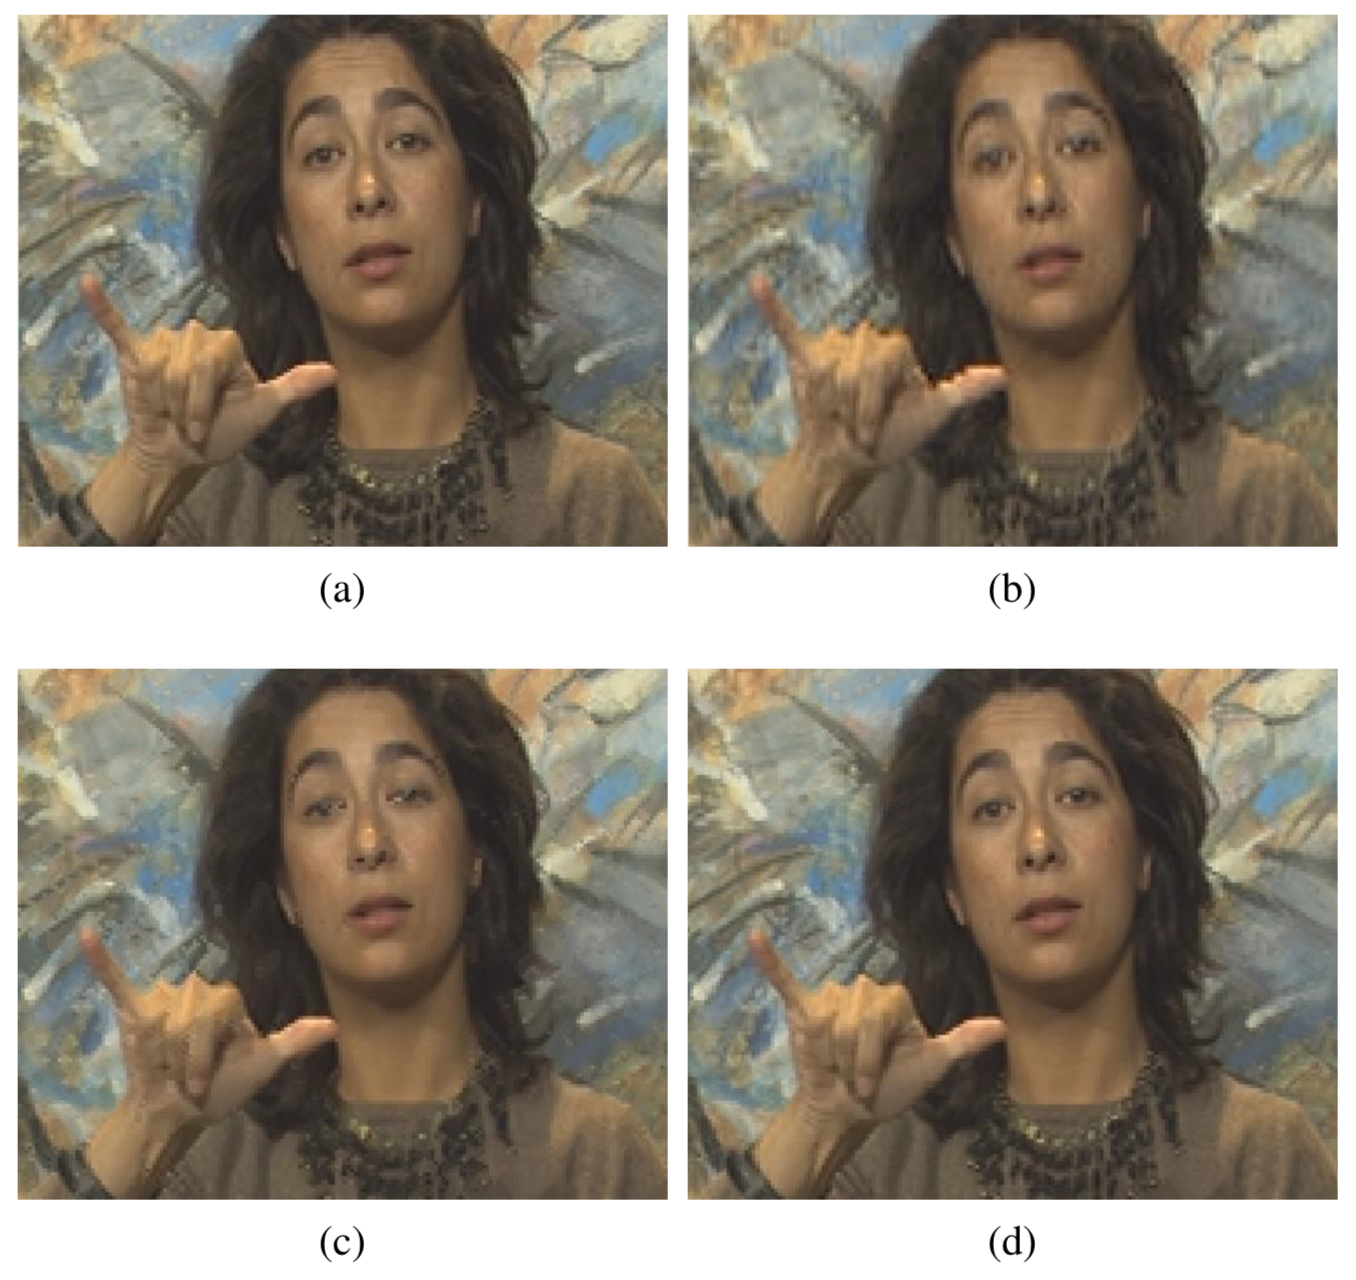
\includegraphics[width=0.8\linewidth]{images/deinterlacing.png}
    \caption{Evaluation of different deinterlacing methods for a frame.
             (a) is the original frame;
             (b) is deinterlaced by the ELA method;
             (c) is deinterlaced by the MNN method; and
             (d) is deinterlaced using locally-adaptive non-local means method.}
    \label{fig:deinterlacing}
\end{figure}
